\documentclass[uplatex,dvipdfmx]{jsarticle}

\usepackage[uplatex,deluxe]{otf} % UTF
\usepackage[noalphabet]{pxchfon} % must be after otf package
\usepackage{stix2} %欧文&数式フォント
\usepackage[fleqn,tbtags]{mathtools} % 数式関連 (w/ amsmath)
\usepackage{hira-stix} % ヒラギノフォント&STIX2 フォント代替定義(Warning回避)


\usepackage{ascmac}
\usepackage{url}
\usepackage{float}
\usepackage{moreverb}
\usepackage{lscape}

\begin{document}

\title{自転車姿勢制御モジュールの提案}
\author{25G1065 塩澤匠生}
\date{2025年6月11日}
\maketitle
\section{はじめに}

社会的背景として自転車の単独事故は年5497件発生していて,その割合は年々増加している
というものがある\cite{jikokensuu}.

そして,
単独事故の原因の内7割が転倒事故であるというものがある\cite{tandokuWariai}.

\subsection{問題点}

ここで,自動車の単独事故の原因の内訳と比較してみると,車の単独事故における転倒(横転)事故の割合は1\%
である一方で,自転車の転倒事故の原因の内7割が転倒事故であることから自転車は乗り物の性質上転倒事故が発生しやすいという問題があると考えることができる.

この問題がなぜ起こるか考えるために,自転車と自動車を比較すると自動車は4輪であるのに対して
自転車は2輪なので,

%一般的な社会的背景を記述したパラグラフを複数配置, パラグラフの終わりは\parを入れる。
%最終パラグラフにはアイデアを記述する.

\subsection{目的}
問題を解決することにより,自転車で転倒事故が発生しない,または発生しにくくすることで
自転車の転倒事故を減少させることを目的とする.

\subsection{主張}

現状,自転車は乗り物の性質上転倒事故が発生するという問題に対して走行中に自転車の転倒を抑制するという製品はない.
そのため今は自転車の転倒事故を減少させるためには呼びかけなどの活動が行われている.

しかし,呼びかけによって乗り手の注意力を高めたとしても急な転倒や
路面状況による転倒など意識するだけでは防ぐことのできない転倒事故がある.

そこで我々は
自転車姿勢制御モジュールというものを提案する.
外付けで物理的に転倒を抑制するモジュールを
提案するこで呼びかけによって転倒に対して
乗り手に注意を促すよりも確実に転倒事故を防止,減少させられることに対する
アプローチになると考えられる.
\section{解決策としての提案手法}

自転車の性質上,転倒事故が発生しやすいという問題に対して我々は自転車姿勢制御モジュールというものを
提案する.自転車姿勢制御モジュールの概念図を図\ref{fig:moduleGainenn}に示す

\begin{figure}[H]
    \centering
    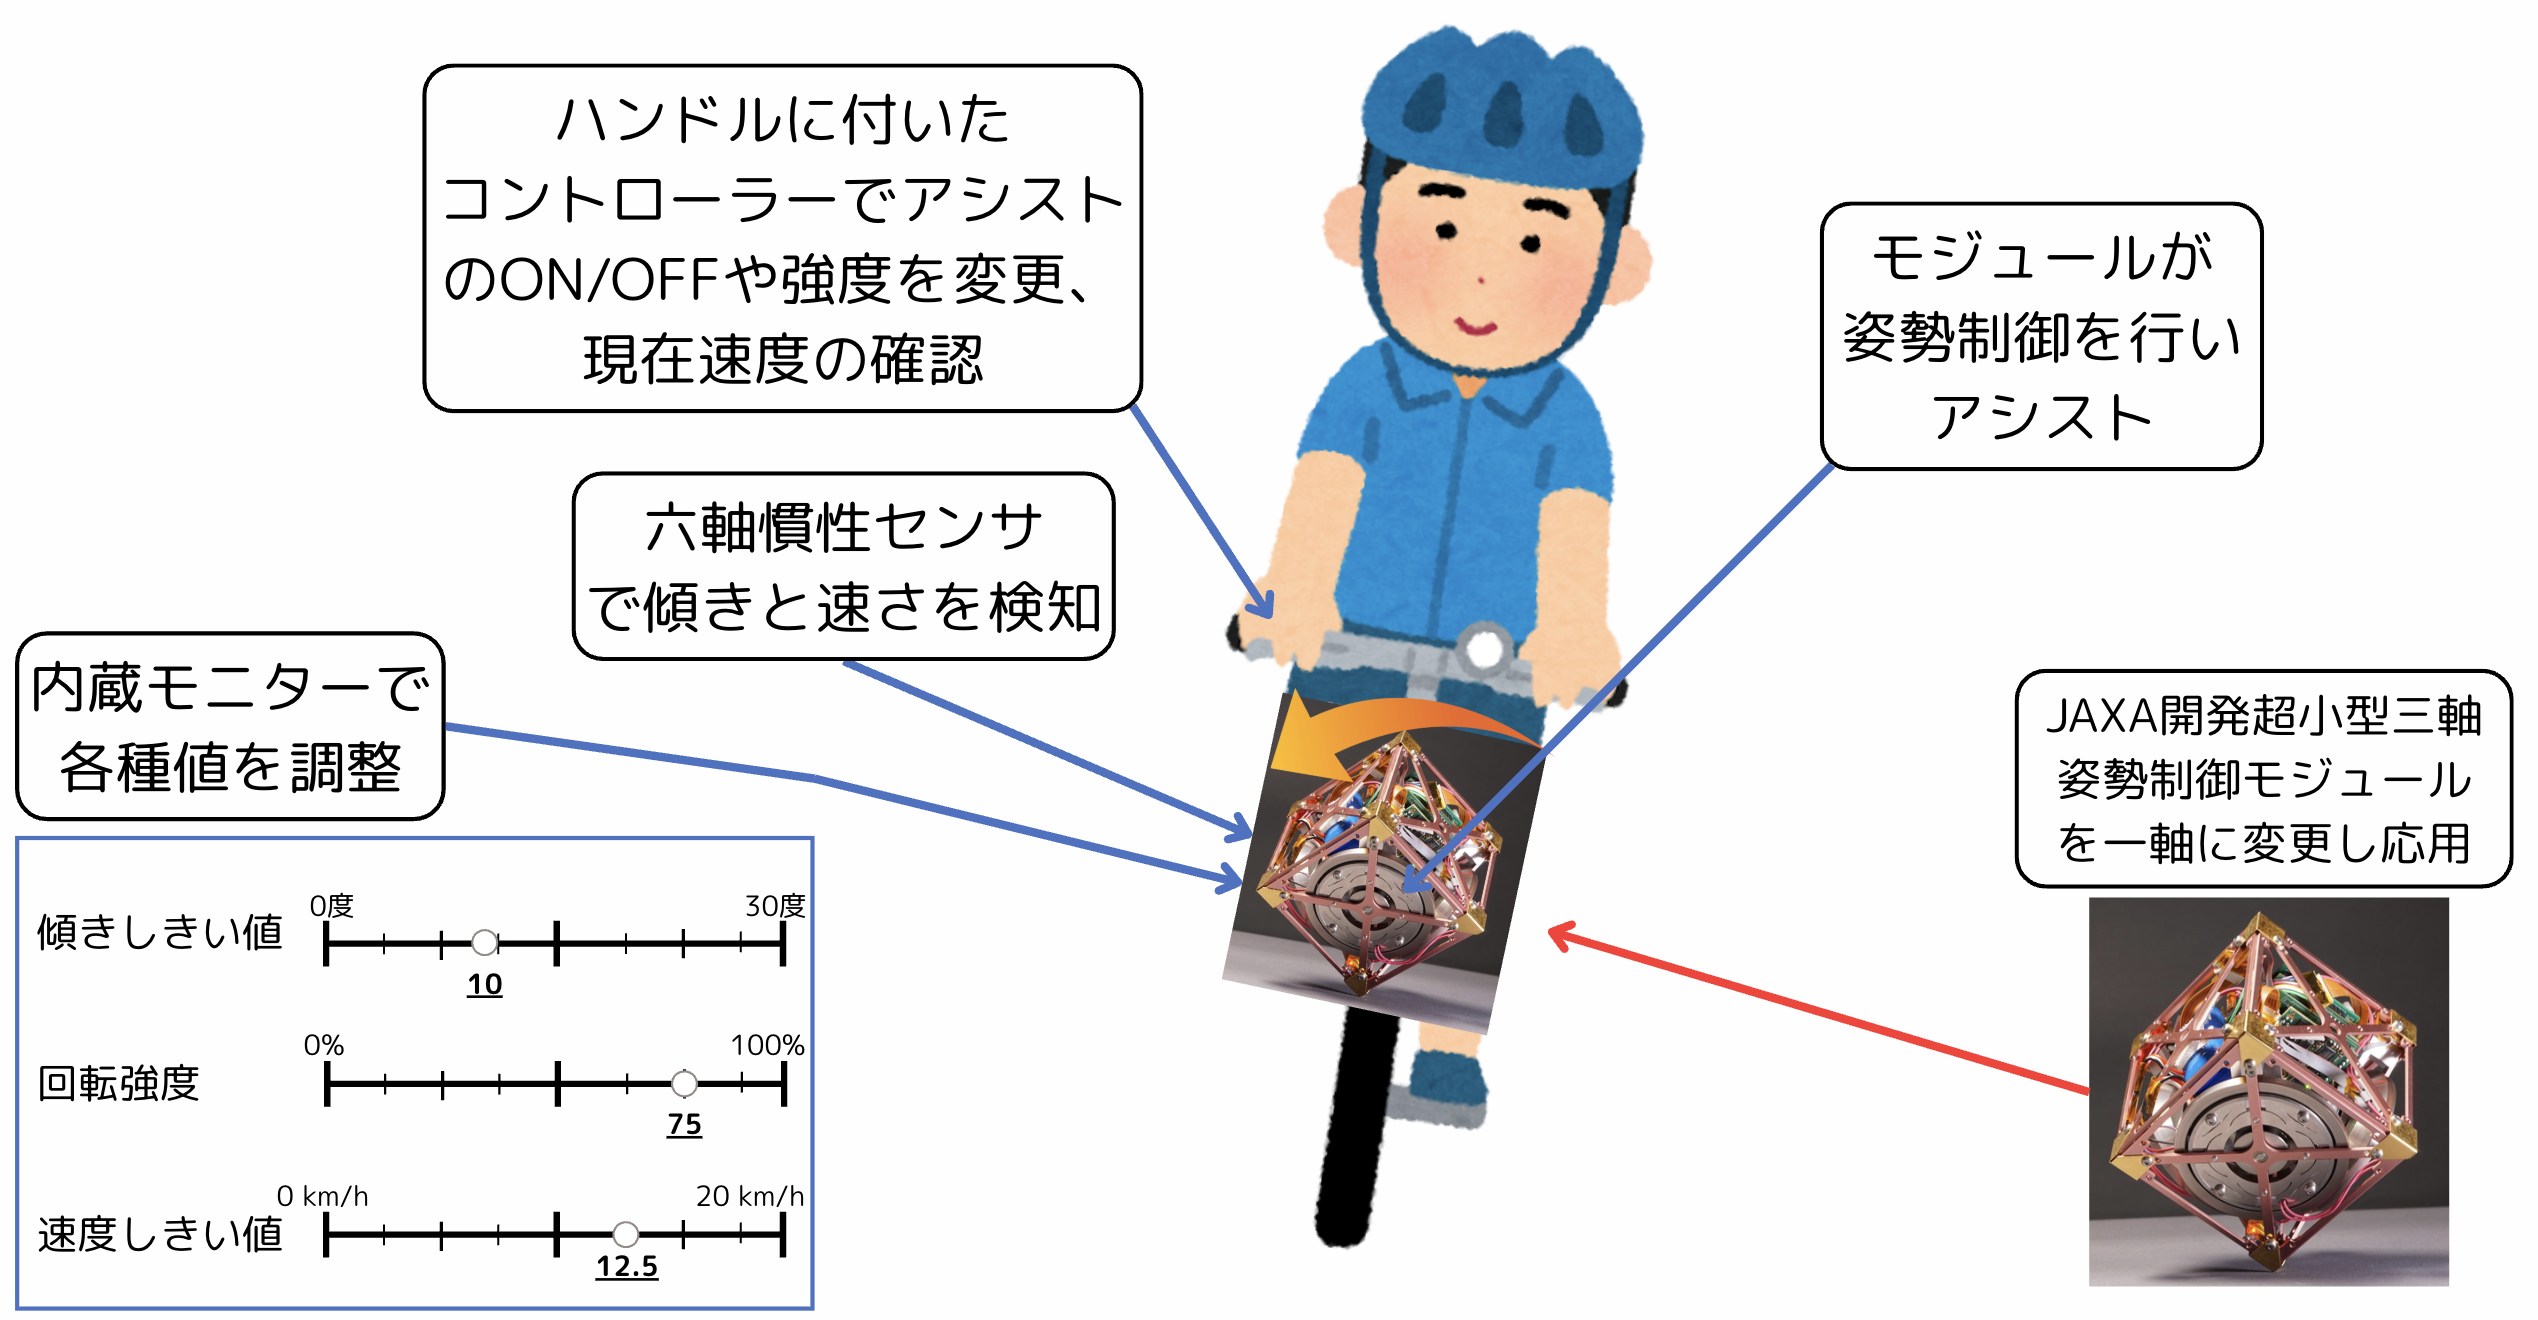
\includegraphics[width=0.8\textwidth]{fig/moduleGainenn2.png}
    \caption{自転車姿勢制御モジュールの概念図}
    \label{fig:moduleGainenn}
\end{figure}

まず,先行研究として,JAXAが開発した超小型三軸姿勢制御モジュールに付いての解説を行う.\cite{jaxaModule}
このモジュールは人工衛星の小型化を図るために作られたもので,慣性センサから本体の傾きを検知し,
ブラシレスDCモータでフライホイールを回転させることで生まれた反作用による力を用いて本体の姿勢を制御するものである.
サイズは$10×10×10 {cm}^3$である.

次に,提案するモジュールに付いての解説を行う.提案する自転車姿勢制御モジュールは先行研究で用いられている技術を応用し,
姿勢制御を行う軸を三軸から一軸に変更することで小型化と軽量化を図り,自転車に搭載しやすくしたモジュールである.
このモジュールは搭載されている六軸慣性センサーにより自転車の傾き,自転車の速度,横方向加速度を取得し,
取得した情報を下にモーターを回転させ,モーターの回転によって生まれる力で自転車の姿勢を保つものである.
また,自転車のハンドル部分にコントローラーを取り付けることで,アシストのON/OFFやアシストの強度変更を運転中に行うことができる
様になっている.このコントローラーには速度のモニター用の速度が有効数字3桁以上で確認できる二色7セグメントLEDもついており,走行速度の確認も同時に行えるように
なっている.この速度モニターは自動アシストが有効になっているか,なっていないかで
表示する色を変える処理を加え,速度の確認とともにアシストが有効になっているかどうかの確認に
ついても行えるようにする.

このモジュールが動作する条件は,低速時に車体のふらつきを検知したとき,急な転倒を検知したとき,
コントローラーからの操作でアシストONが指定されたときの3つである.
低速時に車体のふらつきを検知したときの制御に関しては,アシスト自動OFF速度の設定を行うことにより,
自転車が設定した速度以上に達し,十分車体が安定したと判断される場合は自動でふらつきを検知したときの制御がOFF
になり,車体を傾けてのカーブが可能になる.
急な転倒を検知したときの制御に関しては六軸慣性センサーで車体の横方向の加速度の急激な変化を検知し,
転倒を検知したときに強力なアシストを行う機能である.

検出される傾きのしきい値やモーターの回転力の強さ,アシスト自動OFF速度のしきい値など,
乗る人によって個別に設定が必要な項目についてはモジュールに取り付けられたモニターで細く設定することができる.
自転車後輪上部にある荷台への取り付けを可能にすることで様々な自転車に特別な取り付け器具無しでつけられる様に
することを想定している.

次にモジュールの制御に関する具体的な流れ図を図\ref{fig:nagare}に示す.
\begin{figure}[H]
    \centering
    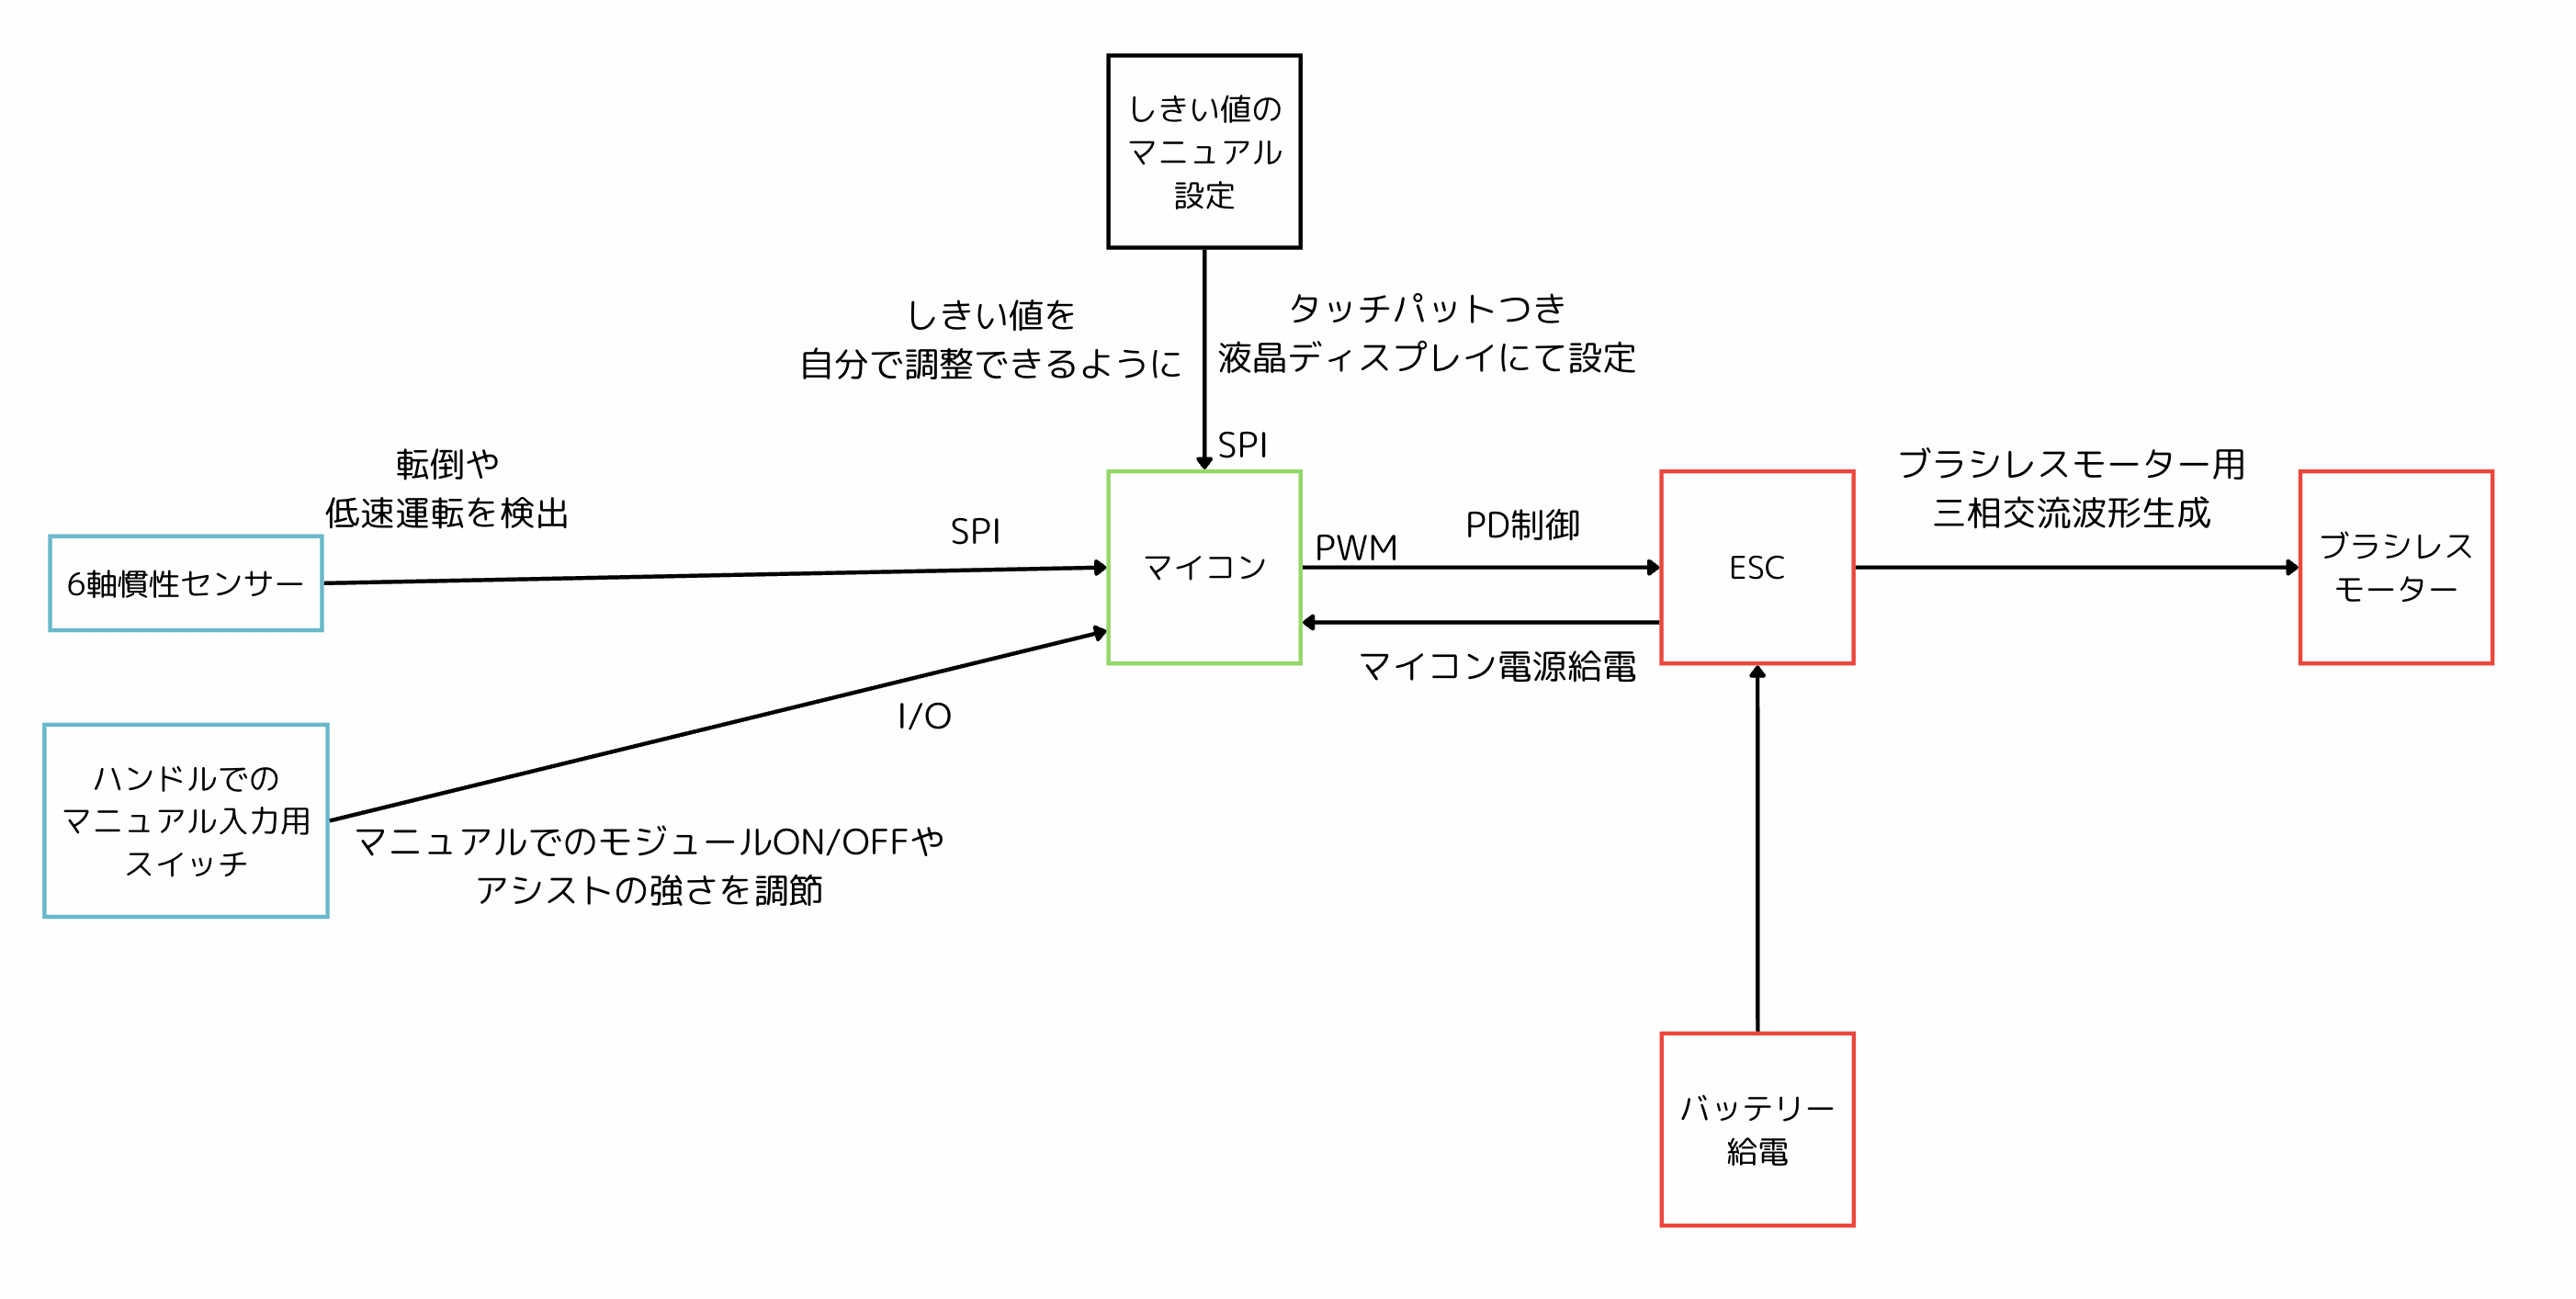
\includegraphics[width=0.9\textwidth]{fig/nagare.png}
    \caption{自転車姿勢制御モジュールの制御の流れ図}
    \label{fig:nagare}
\end{figure}

制御用マイコンへの入力として,6軸慣性センサー,ハンドル部のコントローラーがあり,そのデータ基づいて
マイコンがPID制御を行い,適切なPWM波形を生成し,ESCに対して出力.そしてESCがPWM波形を三相交流電圧
に変換し,ブラシレスモーターを制御するという流れになっている.ここでESCに付いての解説を行う.ブラシレスモーターはDCモーター
と違い,制御するために単純な直流電圧ではなく三相交流電圧が要求される.そこで,PWM波形に基づいて
三相交流波形を生成するものがESCである.

そして次にモジュールを実現するための部品の選定を行った.
まず,6軸慣性センサについては車体の速度検出,車体の傾き検出,そして
急な転倒の検知が求められるのでデータの取得が高速かつデータの精度の高いセンサーが要求される.
そこで今回はPanasonicが販売しているEWTS5Gを使用するのが適切だと考えられる.
EWTS5Gはマイコンとの通信方式が$SPI$であり,他のシリアルの規格である$I^2c$や$UART$
と比べて高速なデータ通信が可能であり,感度出力誤差も$\leq \pm 3.0\%$であることから精度も
申し分ないと考えられるので,自転車姿勢制御モジュールの6軸慣性センサとして適していると考えられる.

自転車の姿勢を保てるほどの強力なモーターに関してはブラシレスモーターを使用するのが適切と考えられる.
ブラシレスモーターはDCモーターに比べ小型でも強い力を生み出すことができるのでこのモジュール
の要件に適している.実験を行ったわけではないのでどのくらいのパワーがあれば
自転車の姿勢制御が十分に行えるかはわからないが,今回はネットで売られている商品の内
なるべく1ボルトあたりの無負荷回転数が高いものを使用する想定にする.無負荷回転数が高ければ,
フライホイールを高速で回し,大きな力を得ることが可能だと考えられる.また,1ボルトあたりの無負荷回転数
が増えるとモーターのトルクが下げるという問題があるが,もしフライホイールを回すためのトルクが足りなかった場合は
減速ギアを使用し,トルクを上げることで対応可能である.
そして,もう一つのブラシレスモーターの選定基準として,センサー付きかという基準を設ける.
ブラシレスモーターにはセンサー付きのものがあり,このセンサー付きのモデルは
ローターの位置を把握する事ができ,これにより,スムーズなモーターの始動制御が可能になる.
自転車姿勢制御モジュールは細かな制御が必要だと考えられるため,このセンサーがついていることは
必須の条件だと考えられる.
これらの基準から部品の選定を行うと1ボルトあたりの無負荷回転数が4150回転と高く,
センサー付きのブラシレスモーターである
ジーフォース社のNeo Fast 8.5Tというモーターを
使用するのが適切であると考えられる.

次にNeo Fast 8.5Tも動かすことができるESCの選定を行った.
Neo Fast 8.5Tは
対応電圧$8.4V$,最大出力$345W$なので電流量$I=W/V$で求めると$I=41A$となり,ESC
の出力できる電流量が$41A$以上のものを搭載しなければならない.また,モーター
始動時の突入電流のことを考慮し選定を行ったところ,
ジーフォース社のBLC50 Type-Dを使用するのが適切だと考えられる.このESCは
連続最大電流が$50A$でブラシレスモーターの電流に耐えることができ,また,瞬間最大電流
が$300A$なので突入電流に対しても十分強いためBLC50 Type-Dを使用するのが適切だと言える.

次にバッテリーに付いて考える.BLC50 Type-Dは$2$セル$7.4V$のリポバッテリーか
4-6セル$4.8〜7.2V$のニッケル水素電池に対応している.
今回はニッケル水素電池に比べて小型でも充電容量が多く,高い電流を流すことのできる
$2$セル$7.4V$のリポバッテリーを使用するものとする.
条件にあう商品を調べたところ,容量も十分なSIGP 2S 7.4Vリチウム電池 6000mAh
という商品が見つかったのでこの商品を使用する想定とする.

マイコンは$SPI$での通信とPWM出力ができるものが要求される.
この条件は昨今のマイコンにはだいたい当てはまるので今回は
なるべく開発しやすく安価で高性能なマイコンを選ぶ.
この条件で考えた場合の販売しているESP32-DEVKITC-32E
を使用するのが望ましい.このマイコンは一枚1,292円と安価かつ
arduinoやPlatformIOといった統合開発環境での開発が可能なので
使用するのに適していると考えられる.

次にしきい値等の調整に用いる液晶モジュールについて考える.
値の調整を行うため外部からの入力が必要だが,タッチパッド機能付きの
液晶を採用すればボタン等の入力機器を搭載しなくてもそれ単体で役割を果たせるため
タッチパッド機能付きの液晶を探す.
十分設定が行えるサイズであることも考慮し,
今回はILI9341搭載2.8インチSPI制御タッチパネル付TFT液晶 MSP2807を使用する想定とする.


\begin{figure}[H]
    \centering
    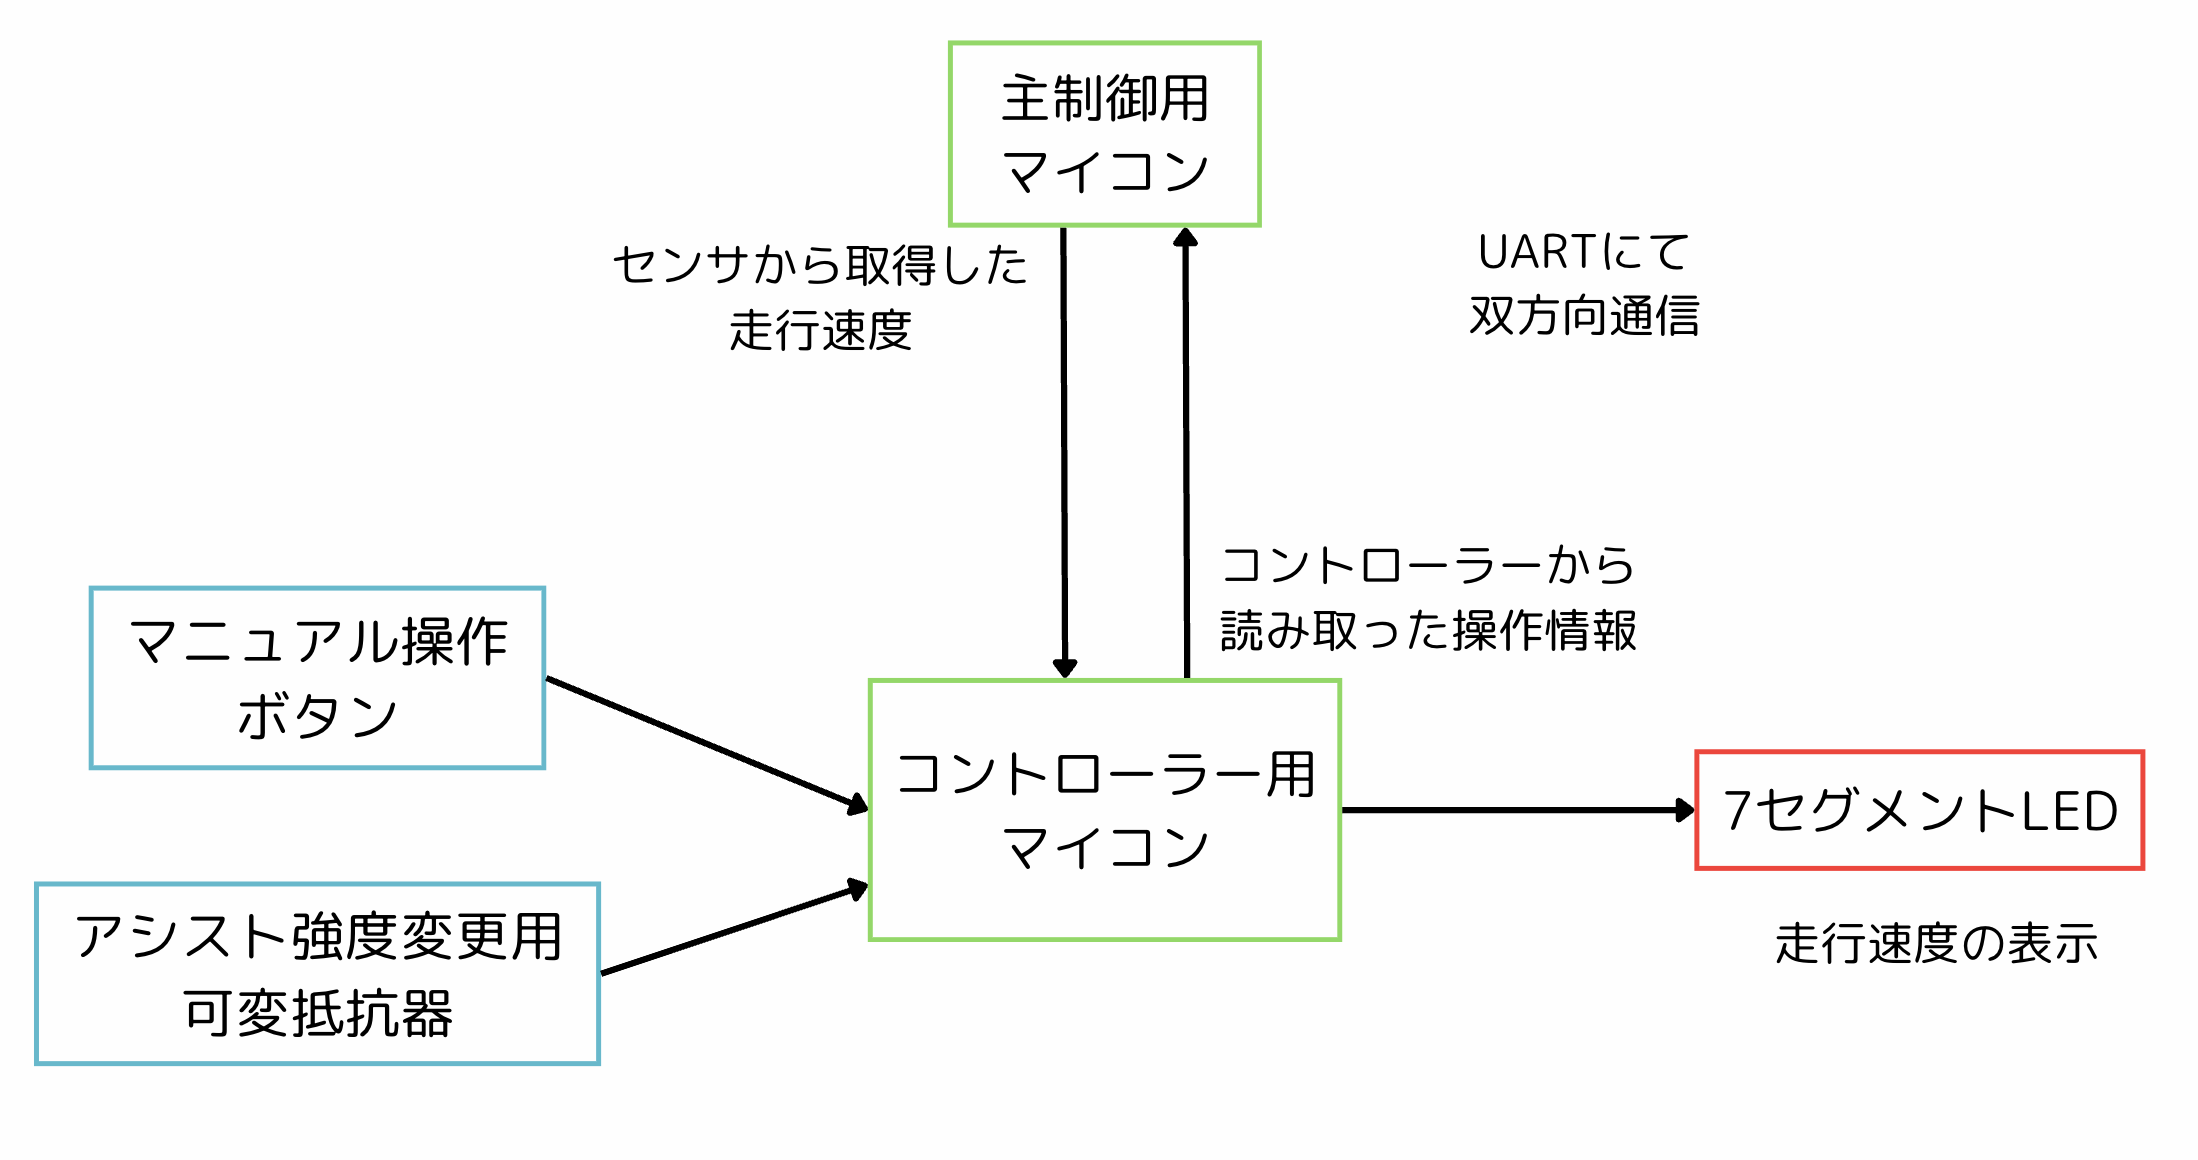
\includegraphics[width=0.9\textwidth]{fig/nagare_conto.png}
    \caption{コントローラー制御の流れ図}
    \label{fig:nagare_conto}
\end{figure}
次にハンドル部のコントローラーに関しての解説を行う.
ハンドル部についての処理の流れ図を図\ref{fig:nagare_conto}に示す.

コントローラーはハンドル部に取り付けられており,主制御部である後輪からは1メートル
ほど離れており,単純にGPIOによりスイッチからの情報を取得しようとすると配線の距離が長いため
ノイズが乗り,正確に値が取得できないというリスクが有る.
そこで今回はコントローラー部にも主制御用マイコンとは別にコントローラー用マイコンを搭載する.
コントローラー用マイコンと主制御用マイコンはUARTにて通信を行う.
$I^2c$は推奨される通信距離が$20~30cm$,$SPI$は$10cm$程度であるため
今回の通信には不向きであるがUARTなら$10m$程度の距離でも通信可能であるため今回の
要件に適している.通信するデータの内容は,主制御用マイコンからコントローラー用マイコンに向けては自転車の
速度,コントローラー用マイコンから主制御用マイコンに向けては入力されたボタンと可変抵抗器の値を送信する.
これによりコントローラーでの速度表示とコントローラーからの操作情報の取得が可能になる.

速度確認用の7セグメントLEDは有効数字3桁以上で速度を表現でき,
かつ2色以上の表示色をもつものが求められる.
そこで表示桁が3桁以上かつ,ドットポイントがあるもので
表示色が2色のものを選ぶ必要がある.
これを下に条件に合う7セグメントLEDを調べた結果
4桁 2色7セグメントLED表示器 赤・黄緑 カソードコモン OSL40363-LRYG
という製品が見つかった.最低3桁でも要件は満たされているが,拡張性に付いて
考慮し,今回は4桁のものを採用する.


\section{提案手法の実現可能性の評価と妥当性の検証}
今回提案したモジュールはフライホイールの回転によって生まれた反作用の力を用いて
自転車の姿勢制御を行うものとなっている.
六軸慣性センサから自転車の速度,傾き,横方向加速度を取得,コントローラーからは
マニュアル操作の受付を行い,それらの情報に基づいてPID制御を行い
適切なPWM波形を出力し,波形に基づいてESCがブラシレスモーターを制御するというものになっている.

ここで,提案するモジュールの実現可能性の評価と妥当性の検証を行う.
実現可能性の評価として適切な部品の選定は済んでいるのでそれらの部品が調達可能であるかについての
考察と,
コストを考えた場合実現可能かについての考察を行う.
妥当性の検証としてコントローラーは必要かについての考察と
既存の自転車姿勢制御システムの研究と比べてこのモジュールを実現する
価値があるかについての考察を行う.そして最後に,この提案をするうえでの課題について考える.


\subsection{部品が調達可能かについての考察}
まず,選定した部品が生産終了,在庫切れで調達が不可能なため
実現できなくなっていないかについての考察を行う.


六軸慣性センサであるPanasonic社のEWTS5Gに関してはDigiKeyでの取り扱いがあり,2025年6月18日現在
1,866個の在庫があるため調達可能である.

ブラシレスモーターに使用するジーフォース社のNeo Fast 8.5Tに関しても2025年6月18日現在
Amazonでの取り扱いがあり,在庫不足の表記もないことから調達可能である.

ESCに使用するジーフォース社のBLC50 Type-Dに関しても2025年6月18日現在
Amazonでの取り扱いがあり,在庫不足の表記もないことから調達可能である.

リポバッテリーに用いるSIGP 2S 7.4V 6000mAhに関しても2025年6月18日現在
Amazonでの取り扱いがあり,在庫不足の表記もないことから調達可能である.

マイコンに使用するEspressif Systems社のESP32-DEVKITC-32Eに関しても2025年6月18日現在
DigiKeyでの取り扱いがあり,
1,183個の在庫があるため調達可能である.

液晶モジュールに使用するMSP2807に関しても2025年6月18日現在
秋月電子通商にて取り扱いがあり701個の在庫があることから,
調達可能である.

7セグメントLEDに用いるOSL40363-LRYGに関しても2025年6月18日現在
秋月電子通商にて取り扱いがあり506個の在庫があることから,
調達可能である.

このことから使用する製品はすべて現在販売されており在庫もあることから
調達可能なためモジュールの開発は実現可能であると考えられる.


\subsection{コストに関する考察}

次に,コスト面に付いての考察を行う.
まずは使用する製品の値段をまとめる.値段は取り扱いを確認した店舗での販売価格を参考にする.
まとめた結果を表\ref{table:Price}に示す.

\begin{table}[h]
  \centering
  \caption{使用を想定する製品の値段表}
  \label{table:Price}
  \begin{tabular}{clr}
\hline
取り扱い店舗 & 製品名 & 値段(円) \\\hline \hline
DigiKey & 6軸慣性センサー(Panasonic EWTS5G) & 2,821 \\\hline
Amazon & ブラシレスモーター(Neo Fast 8.5T) & 7,480 \\\hline
Amazon & ESC(BLC50 Type-D) & 6,530  \\\hline
Amazon & リポバッテリー(SIGP 2S 7.4V 6000mAh) & 4,199 \\\hline
DigiKey & マイコン(ESP32-DEVKITC-32E) & 1,292 \\\hline
秋月電子通商 & 液晶モジュール(MSP2807) & 1,450 \\\hline
秋月電子通商 & 7セグメントLED (OSL40363-LRYG) & 220 \\\hline
  \end{tabular}
\end{table}

マイコンは2つ使用するので2個分の値段で計算し,全ての値段を合計すると以下のようになります。

\begin{align*}
\text{合計金額} &= 2,821 + 7,480 + 6,530 + 4,199 + (1,292 \times 2) + 1,450 + 220 \\
&= 25,284 \, \text{円}
\end{align*}

したがって,提案する自転車姿勢制御モジュールの部品コストは約25,284円となります。
更にここに具体的な金額の算出の難しい項目の金額を追加する.
細かな電子部品(抵抗,コンデンサーなど)やスイッチの値段を1000円程度と仮定し,
外形フレームやフライホイールの値段を10000円程度と仮定すると
約37000円が制作費用にかかると考えられる.

モジュールが様々な自転車に取り付け可能で使いまわしできることから十分妥当な金額だと言える.

\subsection{コントローラーは必要かに付いての考察}

コントローラーは本当に必要かにつての考察を行う.
コントローラーをつける目的としてはマニュアル操作でのアシストON/OFF切り替えと,
アシスト強度の変更,走行速度の確認である.

ここで,コントローラーが無い場合どのような問題があるか考える.
コントローラーが無い場合,まず運転中のマニュアル操作でのアシストON/OFFの
切り替えができなくなる.これが起こってしまうと自分の想定していないタイミング
でアシストがONになってしまった場合とっさにOFFにすることができず,
転倒事故の発生につながってしまうと考えられる.これは転倒事故の減少という
このモジュールの目的と真反対の結果なので,起こってはならない.
また,逆に何らかの要因でアシストが自動でONにならなかった場合
マニュアル操作でONにできないとこちらも転倒事故の減少という
このモジュールの目的から遠ざかってしまうので起こってはならない.
よってマニュアル操作でのアシストON/OFF切り替えは必須の機能だと考えられる.
次に,コントローラーが無い場合,アシスト強度の運転中の変更ができなくなることについて考える.
一見,モーターの回転する強さはモニターから変更ができるためこの機能は不要なものかと
思える.
しかし,この機能がなかった場合,モニターで設定した値が適切でなかった時に
とっさのアシストの強度変更ができなく,アシストが弱すぎたり逆に強すぎたりして
転倒につながってしまうと考えられる.このとき転倒事故の減少という
このモジュールの目的にそぐわなくなるのでこの機能は必要だと考えられる.
しかし,PID制御するなら多少モニターで設定した値が適切でなかったとしても
補正が効くのでは?という考え方もできる.確かに補正がされることで
結果的にはアシストができるかもしれないがPID制御の性質上,適切
に補正がなされるまで補正が完了するまでの遅延が生まれる.これが生まれてしまうと
急な転倒など,即座にアシストが必要な場面で若干の遅れが生じてしまう可能性がある.
これは転倒事故の減少というこのモジュールの目的に対して不確実なものに
してしまう恐れがあるので,目的を確実に達成できるようにするにはこの機能は
確実に必要だと考えられる.

\subsection{既存のジャイロスコープを取り付けた自転車の安定化モジュールとの違い}
製品化はしていないが,芝浦工業大学の研究としてジャイロ制御による自転車転倒防止システム
というものがある.このモジュールとの違いを考察する.

まず,自転車に対する姿勢制御の手段が違う.ジャイロ制御による自転車転倒防止システムはその名の
通りフライホイールが回転し続ける事によって生まれるジャイロ効果を利用して姿勢を制御するものである.
しかし,我々が提案するモジュールは転倒しそうになった場合のみフライホイールを回転させ
回転したときに生じる反作用の力で姿勢を補正するものである.
ジャイロ効果を用いて制御する場合,まずアシストを行いたい場合常にモーターを回転させ続ける
必要がある.この場合,アシストが不必要な場面でもモーターは常に回転し続け,
モーターが発熱することになる.モーターが発熱すると内部抵抗が
増加しモーターの出力が落ちたり,モーターが劣化するという問題がある.
しかし我々の提案するモジュールであれば,アシストが必要な場面のみ適切に
モーターを回転させるという処理方法のためモーターの発熱を最小限に抑えることができる.


ここで,我々の提案するモジュールの欠点についても考える.
ジャイロ効果を用いた場合は単純にモーターを回転させるだけでいいので
自転車の傾きを取得したり複雑なPID制御が不要というメリットが有る.
だが,傾きも取得しないとなると
低速時のみモーターを回すという処理になる.その場合
ある程度速度が出ている状況で急な転倒が発生した場合モーターは
回転しておらず自転車の姿勢の制御ができない.
そのため,ジャイロ効果を用いた場合だと低速時の姿勢の安定化しかできなくなる.

よって,追加のセンサーや複雑な制御が必要な代わりに
急な転倒などのジャイロ効果を用いた場合では対応できないケース
に対応することができるとなると自転車の転倒事故を減少させるという
このモジュールの目的に更に効果的にアプローチでき,モーターを回転させるという処理方法のためモーターの発熱を最小限に抑えること
ができる
我々の提案するフライホイールが回転する事によって生まれる
反作用の力を用いた制御方法の方が優れていると言える.




\subsection{提案する上での課題}
このモジュールを提案するにあたっての課題は2つある.

1つ目はモーターの出力がどの程度あれば自転車の姿勢を保つのに
十分かについての検証を行えていないことである.

今回はなるべく1ボルトあたりの無負荷回転数が高いものを
選ぶという基準で部品の選定を行った.回転数が高ければそれだけ
フライホイールを回す事ができ,より多くの反作用の力を生み出すことができるので
この基準については間違っていないと考えられる.

しかし,その結果選ばれたモーターの1ボルトあたりの無負荷回転数である4150回転
は他のブラシレスモーターと比べて回転数が多いというだけであり,4150回転
あれば自転車の姿勢を制御できるという確実な根拠を示せていない.

2つ目の課題はリポバッテリーの安全性についての課題である.

リポバッテリーは放電性能に優れる一方,過充電をすると発熱や膨張,最悪の場合発火や爆発
が起こるという性質と,過放電をすると内部構造が損傷し,容量が低下したり,
充電ができなくなったりするという性質がある.
そのため適切に充電管理を行う必要があり,知識のない利用者でも
確実にバッテリーを運用することができる必要がある.
しかし,今回はバッテリー充電については考察,想定ができていない.

\section{おわりに}
%全体のまとめを簡潔に記述して,結論を述べる.

今回我々は自転車は乗り物の性質上転倒事故が発生しやすいという問題に対して
自転車の転倒事故を減少させるモジュールの提案を行った.
そこで提案した自転車姿勢制御モジュールはモータによってフライホイールを回転させ
生まれる反作用の力によって自転車の姿勢を制御するものである.

このモジュールが実現すれば自転車の転倒事故の防止,減少をさせることができ,
自転車は乗り物の性質上転倒事故が発生しやすいという問題を解消または
軽減できる.

また,自転車の単独事故は年5497件発生していて,その割合は年々増加している
という社会的背景に対しても,自転車の単独事故が件数の減少することが
期待できる.





\begin{thebibliography}{9}

\bibitem{jikokensuu} NEONAVI, 【自転車事故の実態】を知って安全に利用しよう~令和5年「交通事故統計」から, 
2025年6月11日閲覧,\url{https://neonavi.info/11203/}

\bibitem{tandokuWariai} 東京海上日動, 便利な自転車は運転次第で危険な乗り物になる, 
2025年6月11日閲覧,\url{https://www.tokiomarine-nichido.co.jp/world/guide/drive/202105.html}

\bibitem{jaxaModule} 礒川悌次郎, \& 信川創. (2023). 脳・神経系における機能創発の解明を目指した数理モデリングとデータ駆動分析―局所神経回路から大域的全脳レベルまで―. 計測と制御, 62(10), 587-592.

\end{thebibliography}

\end{document} 
